\documentclass[]{article}
\usepackage[T1]{fontenc}
\usepackage{lmodern}
\usepackage{amssymb,amsmath}
\usepackage{ifxetex,ifluatex}
\usepackage{fixltx2e} % provides \textsubscript
% use upquote if available, for straight quotes in verbatim environments
\IfFileExists{upquote.sty}{\usepackage{upquote}}{}
\ifnum 0\ifxetex 1\fi\ifluatex 1\fi=0 % if pdftex
  \usepackage[utf8]{inputenc}
\else % if luatex or xelatex
  \ifxetex
    \usepackage{mathspec}
    \usepackage{xltxtra,xunicode}
  \else
    \usepackage{fontspec}
  \fi
  \defaultfontfeatures{Mapping=tex-text,Scale=MatchLowercase}
  \newcommand{\euro}{€}
\fi
% use microtype if available
\IfFileExists{microtype.sty}{\usepackage{microtype}}{}
\usepackage[margin=1.0in]{geometry}
\usepackage{longtable,booktabs}
\usepackage{graphicx}
% Redefine \includegraphics so that, unless explicit options are
% given, the image width will not exceed the width of the page.
% Images get their normal width if they fit onto the page, but
% are scaled down if they would overflow the margins.
\makeatletter
\def\ScaleIfNeeded{%
  \ifdim\Gin@nat@width>\linewidth
    \linewidth
  \else
    \Gin@nat@width
  \fi
}
\makeatother
\let\Oldincludegraphics\includegraphics
{%
 \catcode`\@=11\relax%
 \gdef\includegraphics{\@ifnextchar[{\Oldincludegraphics}{\Oldincludegraphics[width=\ScaleIfNeeded]}}%
}%
\ifxetex
  \usepackage[setpagesize=false, % page size defined by xetex
              unicode=false, % unicode breaks when used with xetex
              xetex]{hyperref}
\else
  \usepackage[unicode=true]{hyperref}
\fi
\hypersetup{breaklinks=true,
            bookmarks=true,
            pdfauthor={},
            pdftitle={},
            colorlinks=true,
            citecolor=blue,
            urlcolor=blue,
            linkcolor=magenta,
            pdfborder={0 0 0}}
\urlstyle{same}  % don't use monospace font for urls
\setlength{\parindent}{0pt}
\setlength{\parskip}{6pt plus 2pt minus 1pt}
\setlength{\emergencystretch}{3em}  % prevent overfull lines
\setcounter{secnumdepth}{0}

\author{}
\date{\vspace{-2.5em}}
\usepackage{helvet}
\renewcommand*\familydefault{\sfdefault}
\usepackage{setspace}
\doublespacing
\usepackage[left]{lineno}
\linenumbers
\usepackage{multirow}
\usepackage{booktabs}
\usepackage{longtable}
\usepackage{array}
\usepackage{multirow}
\usepackage{wrapfig}
\usepackage{float}
\usepackage{colortbl}
\usepackage{pdflscape}
\usepackage{tabu}
\usepackage{threeparttable}
\usepackage{threeparttablex}
\usepackage[normalem]{ulem}
\usepackage{makecell}
\usepackage{xcolor}

\begin{document}

\section{Taxonomic Resolution Matters for Microbiome-Based
Classification of Colorectal
Cancer}\label{taxonomic-resolution-matters-for-microbiome-based-classification-of-colorectal-cancer}

\vspace{10mm}

Courtney R. Armour${^1}$, Begüm D. Topçuoğlu$^{1,2}$, Andrea
Garretto${^1}$, Patrick D. Schloss ${^1}$${^*}$

\vspace{5mm}

${^1}$ Department of Microbiology and Immunology, University of
Michigan, Ann Arbor MI

${^2}$ Exploratory Science Center, Merck \& Co., Inc., Cambridge,
Massachusetts, USA~

\vspace{5mm}

${^*}$ Correspondence: Patrick D. Schloss
\href{mailto:pschloss@umich.edu}{pschloss@umich.edu}

\vspace{20mm}

\textbf{observation format}

\newpage

\subsubsection{Abstract}\label{abstract}

Colorectal cancer is a common and deadly disease in the United States
accounting for over 50,000 deaths in 2020. This progressive disease is
highly preventable with early detection and treatment, but many people
do not comply with the recommended screening guidelines. The gut
microbiome has emerged as a promising target for non-invasive detection
of colorectal cancer. Most microbiome-based classification efforts
utilize taxonomic abundance data from operational taxonomic units (OTUs)
or amplicon sequence variants (ASVs). However, it is unknown which
taxonomic resolution is optimal for microbiome-based classification of
colorectal cancer. To address this question, we used a reproducible
machine learning framework to quantify classification performance of
models based on data annotated to phylum, class, order, family, genus,
OTU, and ASV levels. We found that model performance increased with
increasing taxonomic resolution, up to the family level where
performance was equal among family, genus, and OTU data before
decreasing at the ASV level. These results are a step towards optimizing
a microbiome based diagnostic tool.

\subsubsection{Importance}\label{importance}

Despite being highly preventable, colorectal cancer remains a leading
cause of cancer related death in the United States. Low-cost,
non-invasive detection methods could greatly improve our ability to
identify and treat early stages of disease. While the microbiome has
shown promise as a diagnostic tool, there are numerous details to refine
before a diagnostic could be widely deployed. Among these are the need
for standardization of sample collection, storage, processing, and
analysis. We address one aspect of data analysis by examining which
taxonomic level provides the optimal resolution for microbiome-based
classification of colorectal cancer. This is an important step to inform
the development of microbiome-based diagnostic tools.

\newpage

Colorectal cancer is one of the most common cancers in men and women and
a leading cause of cancer related deaths in the United States (1). Early
detection and treatment are essential to increase survival rates, but
for reasons such as invasiveness and high screening costs
(i.e.~colonoscopy), many people do not comply with recommended screening
guidelines (2). This prompts a need for low cost, non-invasive detection
methods. A growing body of research points to the gut microbiome as a
promising target for non-invasive detection of screen relevant neoplasia
(SRNs) consisting of advanced adenomas and carcinomas (3, 4). The
diagnostic potential of the gut microbiome in detecting SRNs has been
explored through machine learning (ML) methods using abundances of
operational taxonomic unit (OTU) classifications based on amplicon
sequencing of the 16S rRNA gene (3). Recent work has pushed for the use
of amplicon sequence variants (ASVs) to replace OTUs for marker-gene
analysis because of the improved resolution with ASVs (5). However, it
is unclear if OTUs are the optimal taxonomic resolution for classifying
SRNs from microbiome data or whether the additional resolution provided
by ASVs is useful for ML classification. Topçuoğlu \emph{et al} (6)
recently demonstrated how to effectively apply machine learning (ML)
methods to microbiome based classification problems and developed a
framework for applying ML practices in a more reproducible way
(mikropml). This analysis utilizes the reproducible framework developed
by Topçuoğlu \emph{et al} to determine which ML method and taxonomic
level produce the best performing classifier for detecting SRNs from
microbiome data.

Utilizing publicly available 16S rRNA sequence data from stool of
patients with SRNs and healthy controls, we generated taxonomic
abundance tables with mothur (7) annotated to phylum, class, order,
family, genus, OTU and ASV levels. Using the taxonomic abundance data
and the mikropml R package (8), we quantified how reliably samples could
be classified as SRN or normal using five machine learning methods
including random forest, L2-regularized logistic regression, decision
tree, gradient boosted trees (XGBoost), and support vector machine with
radial basis kernel (SVM radial). Across the five machine learning
methods tested, model performance increased with increasing taxonomic
level usually peaking around genus/OTU level before dropping off
slightly with ASVs (Supplemental Figure 1). Regardless of the taxonomic
level, random forest (RF) models consistently had the largest area under
the receiver operating characteristic curve (AUROC). Within the RF
model, the highest AUROCs were observed for family (mean AUROC: 0.689),
genus (mean AUROC: 0.690), and OTU (mean AUROC: 0.693) level data with
no significant difference between the three (Figure 1A, Supplemental
Figure 2). Performance with ASVs (mean AUROC: 0.676) was significantly
lower than OTUs (p \textless{} 0.01), but comparable to family (p =
0.06) and genus (p = 0.05) levels (Figure 1A). These results suggest
that increased resolution improves model performance up to the OTU level
where further taxonomic resolution is not necessarily better for
identifying individuals with SRNs based on microbiome composition.

While comparing AUROC values between models is a useful way to assess
the overall model performance, they summarize the performance across all
thresholds and can be misleading since models with the same AUROC can
have different ROC curve shapes (9). Depending on the intended
implementation of the model, one may want to optimize the true-positive
rate (sensitivity) over the false-positive rate (1-specificity) or vice
versa. In this case, the optimal model will detect as many true
positives (people with SRNs) as possible. To further compare the model
performance across taxonomic levels we compared the sensitivity of the
models at a specificity of 90\%. The highest sensitivity values were
observed for family, genus, and OTU level data (Figure 1B), consistent
with the AUROC results. Phylum, class, order, and ASV sensitivity values
were all significantly lower than family, genus, and OTU sensitivity
values (Figure 1B). This analysis further supports the observation that
finer resolution does not improve SRN detection.

One hypothesis for the observation that model performance increases from
phylum to OTU level then drops slightly at ASV level is that at higher
taxonomic levels (e.g.~phylum) there are too few taxa and too much
overlap to reliably differentiate between cases and controls. At the
level of genus or OTU there is enough data and variation but at the ASV
level, the data is too specific to individuals and does not overlap
enough. Examination of the prevalence of taxa in samples at each level
supports this idea. A majority of taxa were present in greater than 70\%
of samples at the phylum (67\% of taxa) and class (63\% of taxa) levels.
The opposite was observed at the OTU and ASV level where 50\% and 41\%
of taxa, respectively, were only present in 20\% or less of the samples
(Supplemental Figure 3). Of note, the ML pipeline includes a
pre-processing step that occurred prior to training and classifying the
ML models. For example, perfectly correlated taxa provide the same
information to build the model and thus can be collapsed. Additionally,
features with zero or near-zero variance across samples were removed.
Interestingly, despite starting with 104,106 ASVs, only 478 (0.5\%)
remained after pre-processing. At the OTU level, 705 of the 20,079 OTUs
(3.5\%) remained after preprocessing (Table 1). While the resolution
provided by ASVs is useful in certain contexts(10, 11), these results
suggest that the resolution is too fine for use in machine learning
classification of SRNs based on microbiome composition.

A look into the most important taxa at each level for classifying
samples revealed some nesting where several genera and their higher
taxonomic classifications were in the top 10 most important taxa
(Supplemental Figure 4). For example, the genus \emph{Gemella} was an
important taxon at the genus and OTU levels and its higher
classifications were also important (\emph{Firmicutes} \textgreater{}
\emph{Bacilli} \textgreater{} \emph{Bacillales} \textgreater{}
\emph{Bacillales Incertae Sedis XI} \textgreater{} \emph{Gemella}).
\emph{Fusobacterium} displayed a similar pattern, except that the family
level classification (\emph{Fusobacteriaceae}) importance was ranked
16th out of 54 families. In the case of unclassified
\emph{Lachnospiraceae}, there were several OTUs with this label that
were in the top 10, however at the genus level this taxon was ranked
lower in importance (21st out of 115 genera) suggesting there may be
some benefit to separating different taxonomic groupings within
\emph{Lachnospiraceae}.

These results demonstrate that consideration of the appropriate
taxonomic resolution for utilizing the microbiome as a predictive tool
is warranted. In general, we found that finer taxonomic resolution
(e.g.~OTU and ASV) did not add additional sensitivity to predicting SRNs
based on microbiome composition. Family, genus, and OTU level data all
performed equally. At the ASV level the fine resolution actually impedes
model performance due to the sparsity of shared taxa and led to
decreased model performance. The tendency for ASV level annotation to
split single bacterial genomes into multiple taxa (12) could also be a
contributing factor to the sparsity of shared taxa. Overall, either
family, genus, or OTU level taxonomy appear to perform equally for
predicting subjects with SRNs based on the composition of the gut
microbiome. A potential benefit of utilizing genus or family level data
could be that it may allow for merging data generated from different 16S
rRNA gene regions or sequencing platforms.

\subsubsection{Materials and Methods}\label{materials-and-methods}

\textbf{\emph{Dataset.}} Raw 16S rRNA gene amplicon sequence data
isolated from human gut samples (13) was downloaded from NCBI Sequence
Read Archive (SRP062005). This dataset contains stool samples from 490
subjects. Based on the available metadata, samples categorized as
normal, high risk normal, or adenoma were labeled ``normal'' for this
analysis and samples categorized as advanced adenoma or carcinoma were
labeled as ``screen relevant neoplasia'' (SRN). This resulted in a total
of 261 ``normal'' samples and 229 ``SRN'' samples.

\textbf{\emph{Data processing.}} Sequence data was processed with mothur
(1.44.3) (7) using the SILVA reference database (v132) (14) to produce
count tables for phylum, class, order, family, genus, OTU, and ASV
following the Schloss Lab MiSeq SOP described on the mothur website
(\url{https://mothur.org/wiki/miseq_sop/}). ASV level data was also
produced using DADA2 (15) to ensure consistent results with a different
pipeline. Data was processed following the DADA2 pipeline, but setting
pool=TRUE to infer ASVs from the whole dataset rather than per sample.
The resulting ASV table was subsampled for consistency with the mothur
data. The results were consistent for ASVs generated with DADA2 (mean
AUROC: 0.659).

\textbf{\emph{Machine Learning.}} Machine learning models were run with
the R package mikropml (v0.0.2) (8) to predict the diagnosis category
(normal vs SRN) of each sample. Data was preprocessed to normalize
values (scale/center), remove values with zero or near-zero variance,
and collapse collinear features using default parameters. Initially the
models were run with default hyperparameters, but were expanded if the
peak performance was at the edge of the hyperparameter range. Each
taxonomic model taxonomic level combination (e.g.~random forest on
genus) was run with 100 different seeds. Each seed split the data into a
training (80\%) and testing (20\%) set, and output performance of the
training and testing as area under the receiver operating curve (AUROC).

To compare performance between taxonomic levels and models, P values
were calculated as previously described (6). To compare sensitivity at
90\% specificity, probabilities on the test dataset were collected for
each seed and used to calculate sensitivity for specificity values
ranging from 0 to 1 in 0.01 increments. The sensitivity at a specificity
of 90\% was pulled for each seed. The averaged ROC curves were plotted
by taking the average and standard deviation of the sensitivity at each
specificity value. An optional output from the mikropml package is the
permuted feature importance which is quantified by iteratively permuting
each feature in the model and assessing the change in model performance.
Features are presumed to be important if the performance of the model,
measured by the AUROC, decreases when that feature is permuted. Ranking
of feature importance was determined by ordering the features based on
the average change in AUROC across the 100 seeds where features with a
larger decrease in AUROC are ranked higher in importance.

To quantify prevalence of the features, the number of samples with
non-zero abundance was divided by the total number of samples resulting
in values ranging from 0 to 1 where 0 indicates the feature is not found
in any samples, 0.5 indicates the feature is found in half of the
samples, and 1 indicates the feature is found in all of the samples.

All code is available at: \textbf{TODO: link to code}

\subsubsection{Acknowledgements}\label{acknowledgements}

This work was supported through a grant from the NIH (R01CA215574).

\newpage

\subsubsection{References}\label{references}

::: \{\#refs\} :::

\newpage

\subsubsection{Figures}\label{figures}

\begin{figure}[htbp]
\centering
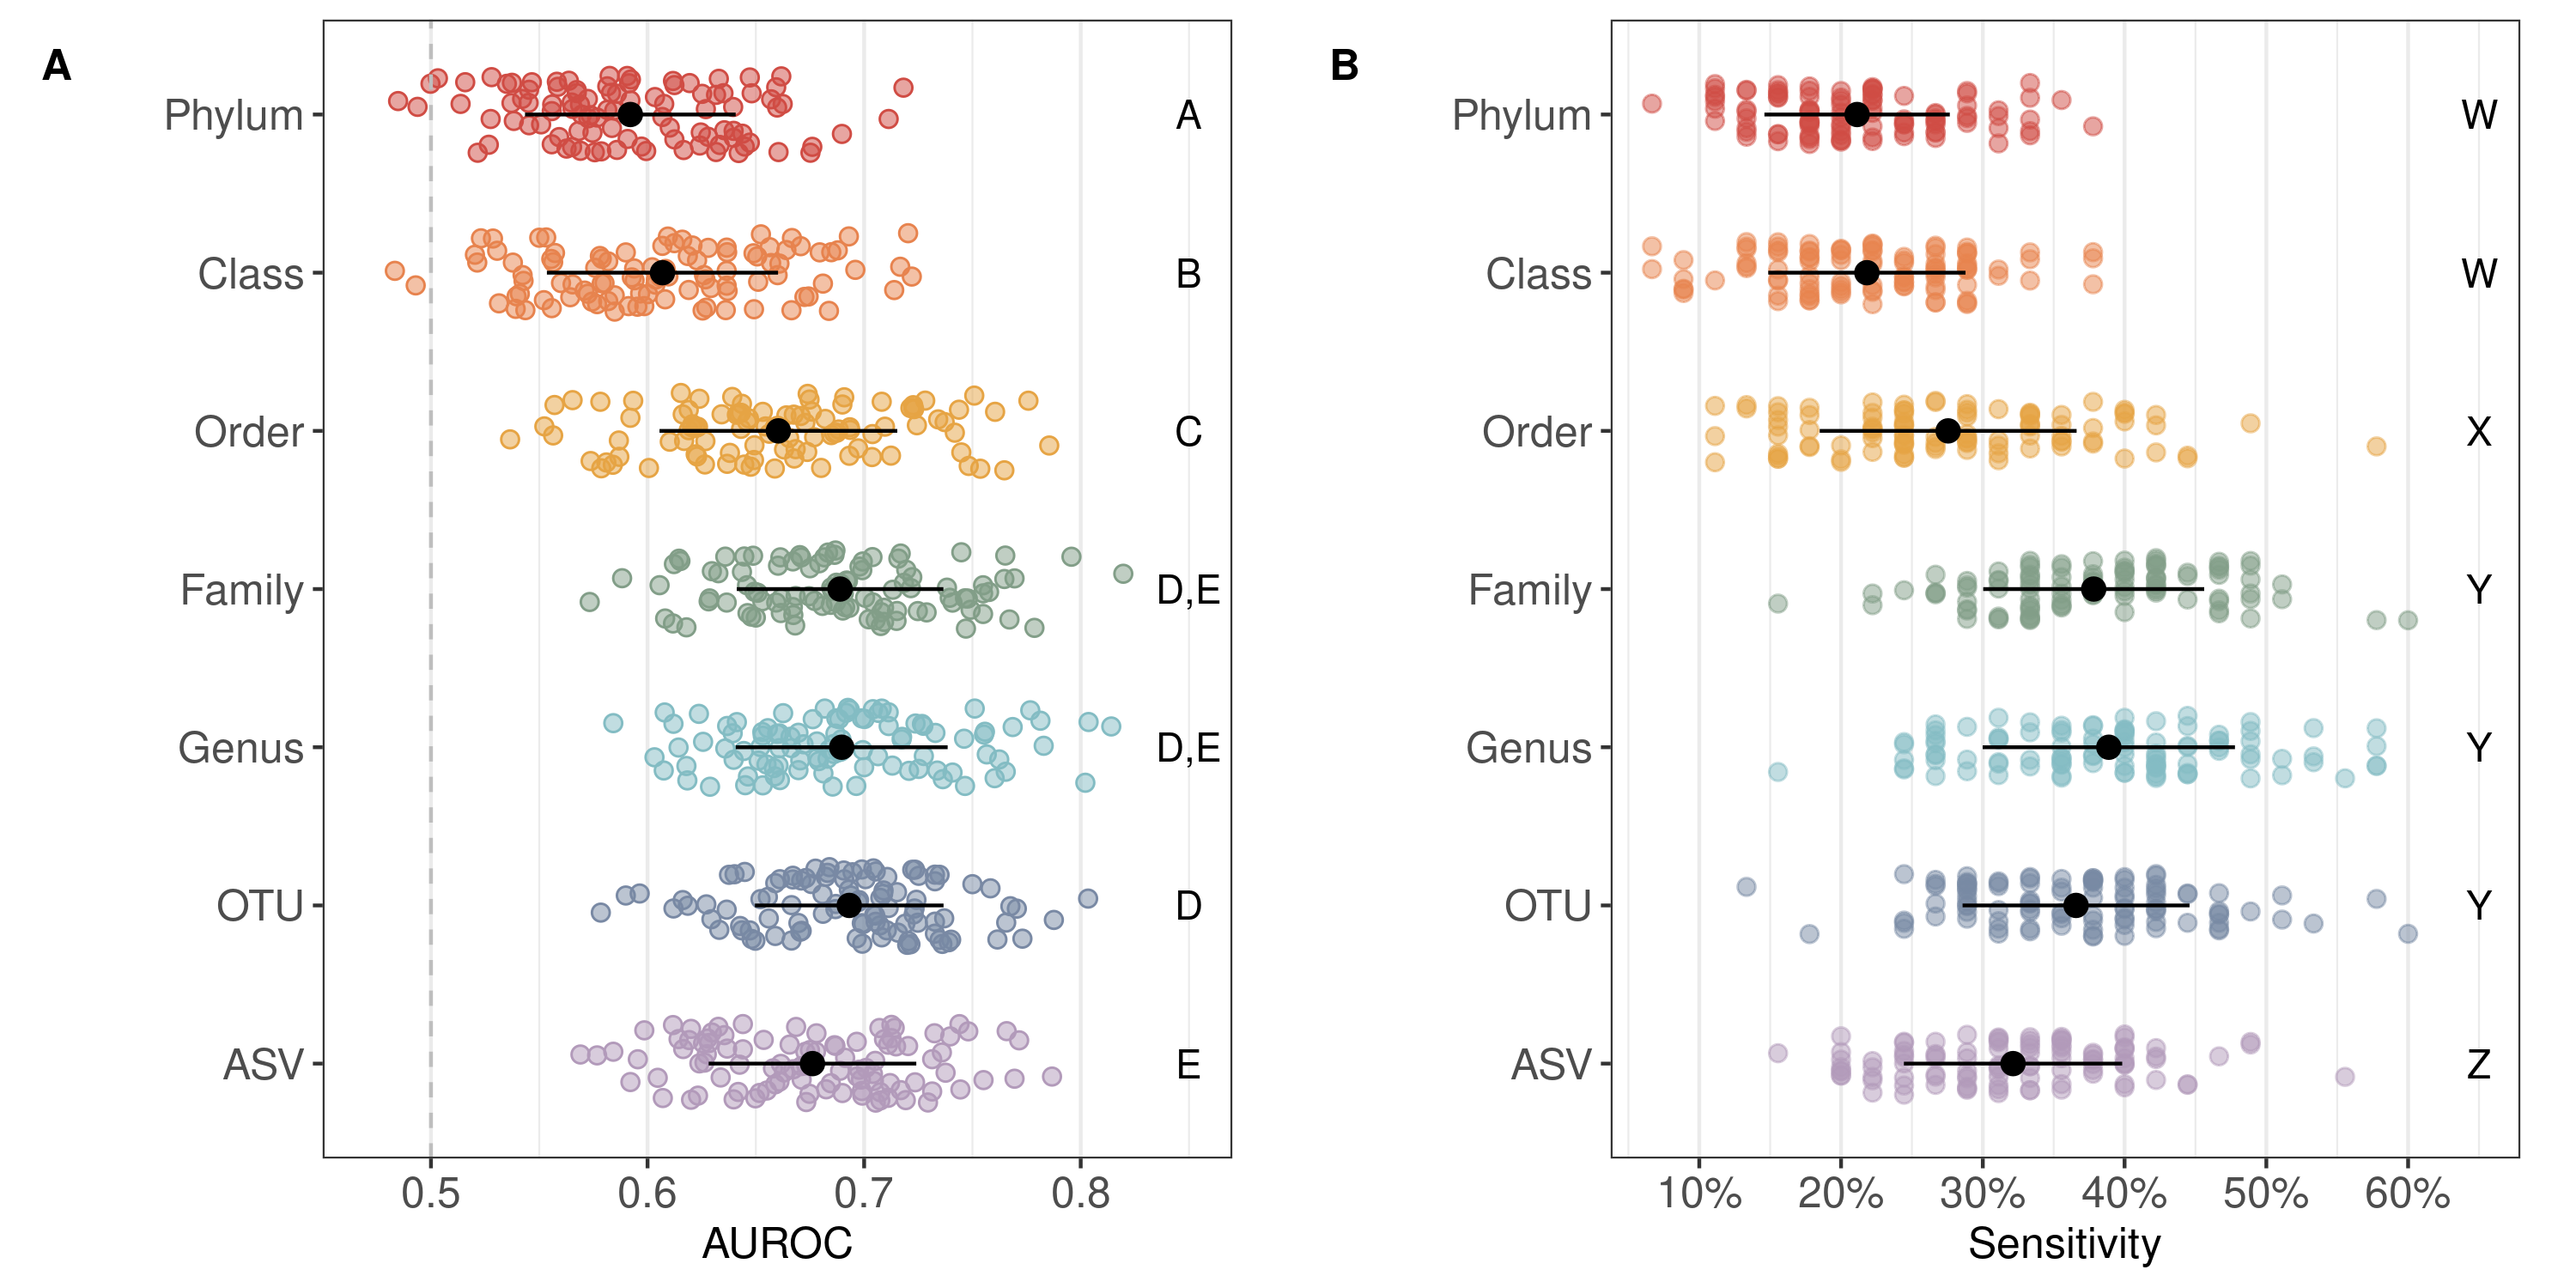
\includegraphics{figure_1.png}
\end{figure}

\textbf{Figure 1: Random Forest Model Performance.} \textbf{A)} Strip
plot of the area under the receiver operating characteristic curve
(AUROC) values on the test dataset for 100 seeds predicting SRNs using a
random forest model. Black points denote the mean and lines denote the
standard deviation. Dashed line denotes AUROC of 0.5 which is equivalent
to random classification. Significance between taxonomic levels was
quantified by comparing the difference in mean AUROC and is denoted by
letters A through E on the right side of the plot; taxonomic levels with
the same letter are in the same significance group and are not
significantly different from one another. \textbf{B)} Strip plot of the
sensitivity at a specificity of 90\% across the 100 model iterations for
each taxonomic level. Black points denote the mean and the lines denote
the standard deviation. The letters W through Z on the right side of the
plot denote the significance groups.

\newpage

\subsubsection{Tables}\label{tables}

\begin{longtable}[c]{@{}lrrc@{}}
\toprule\addlinespace
Taxonomic Level & Number of Features &
\makecell[c]{Number of Features \\ After Preprocessing} &
\makecell[c]{Percent of Features Kept \\ After Preprocessing}
\\\addlinespace
\midrule\endhead
Phylum & 19 & 9 & 47.4 \%
\\\addlinespace
Class & 36 & 19 & 52.8 \%
\\\addlinespace
Order & 65 & 28 & 43.1 \%
\\\addlinespace
Family & 124 & 54 & 43.5 \%
\\\addlinespace
Genus & 316 & 115 & 36.4 \%
\\\addlinespace
OTU & 20,079 & 705 & 3.5 \%
\\\addlinespace
ASV & 104,106 & 478 & 0.5 \%
\\\addlinespace
\bottomrule
\end{longtable}

\textbf{Table 1: Summary of Features.} Overview of the number of
features at each taxonomic level before and after preprocessing as
described in the methods.

\newpage

\subsubsection{Supplemental Figures}\label{supplemental-figures}

\begin{figure}[htbp]
\centering
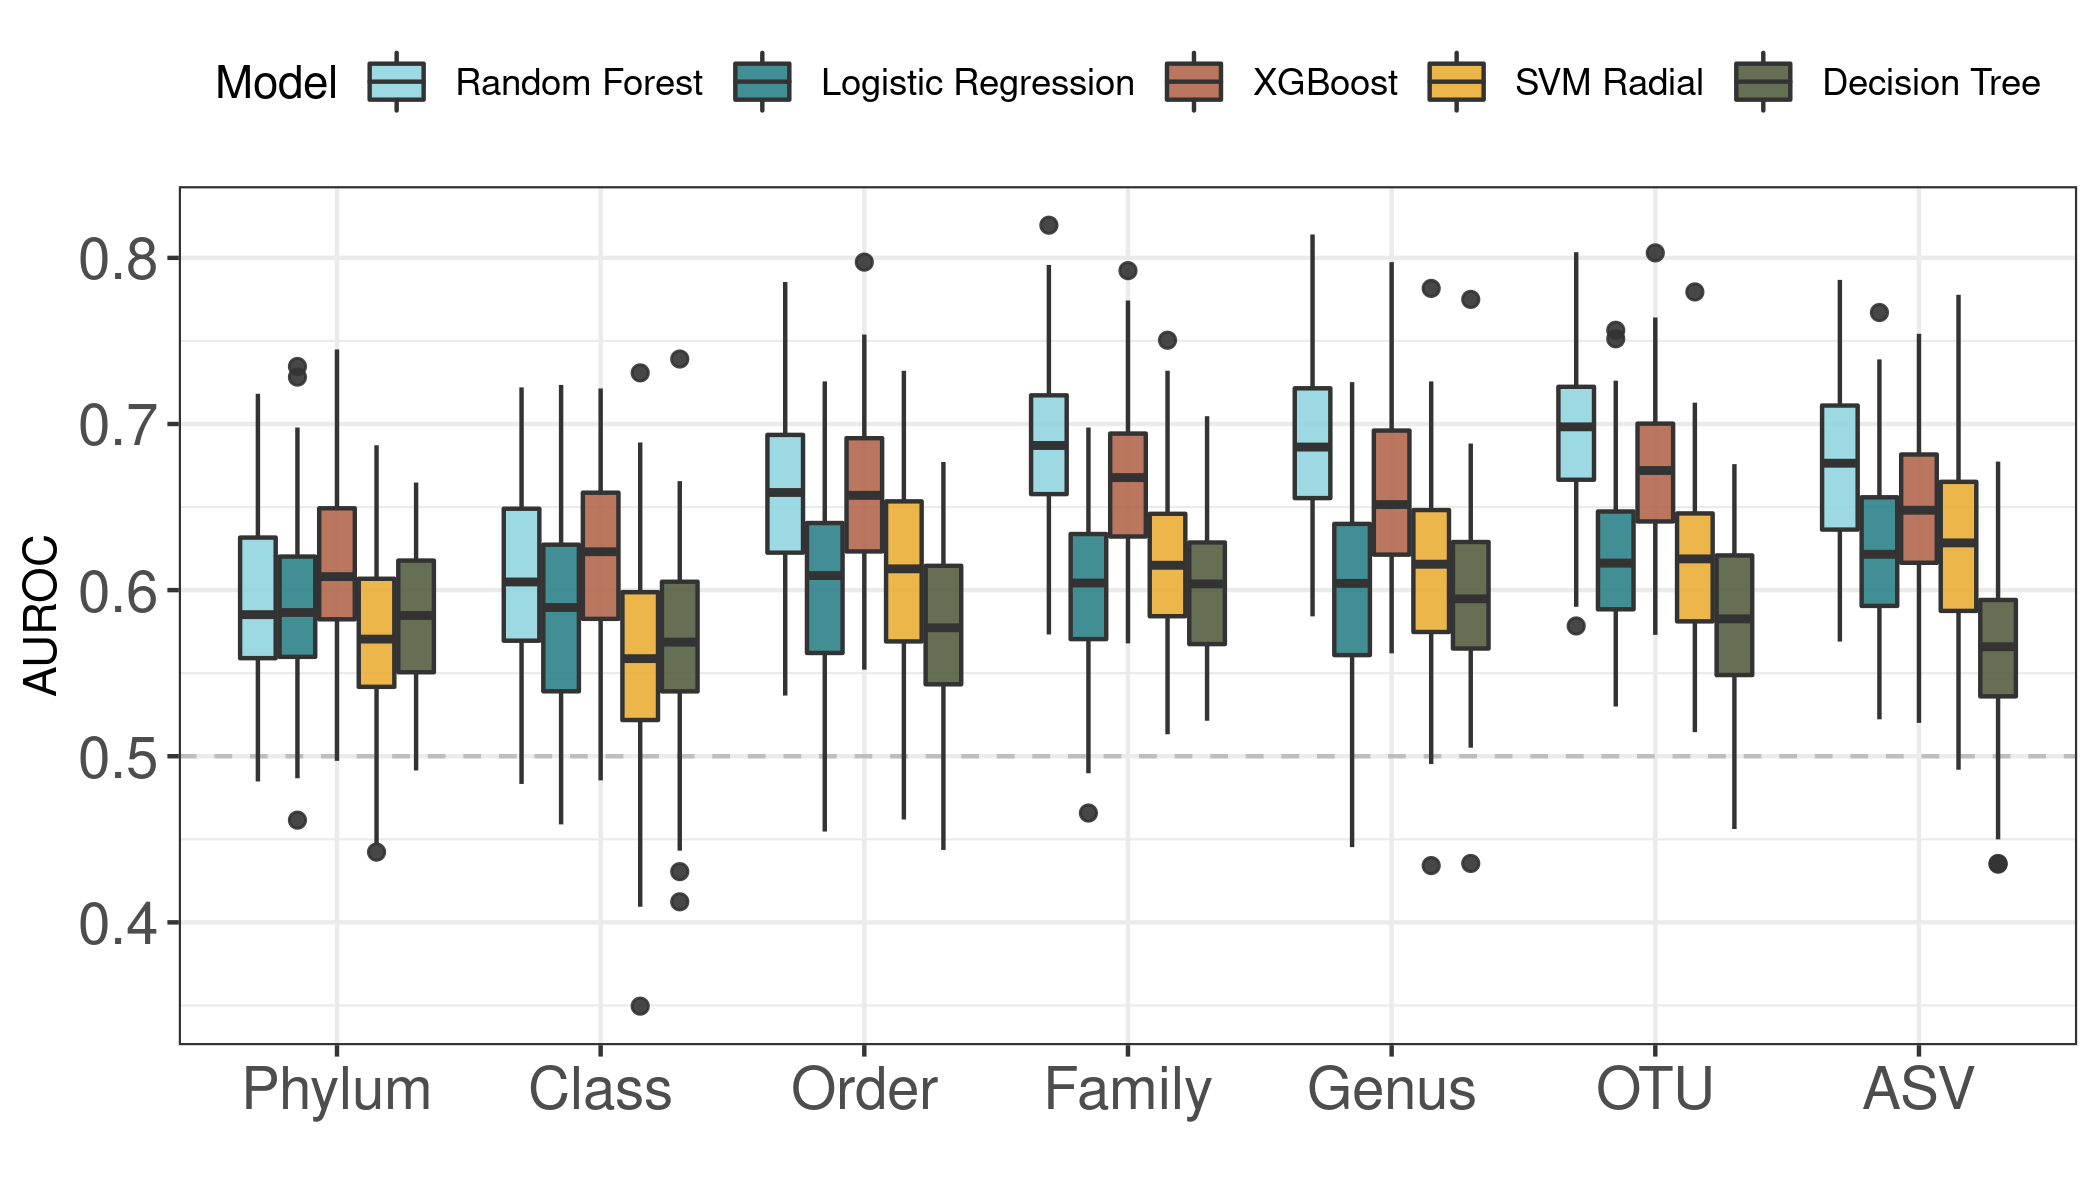
\includegraphics{figure_s1.png}
\end{figure}

\textbf{Supplemental Figure 1: Model Performance across Taxonomy.}
Boxplots of AUROC values from predicting whether samples came from
subjects with screen relevant neoplasias (i.e.~advanced adenoma or
cancer) or healthy controls across five machine learning methods
including random forest, L2-regularized logistic regression (logistic
regression), decision tree, gradient boosted trees (XGBoost), and
support vector machine with radial basis kernel (SVM radial). Due to the
random split of data into training and testing sets, each model was run
across 100 seeds to account for variation in training/test datasplits.

\newpage

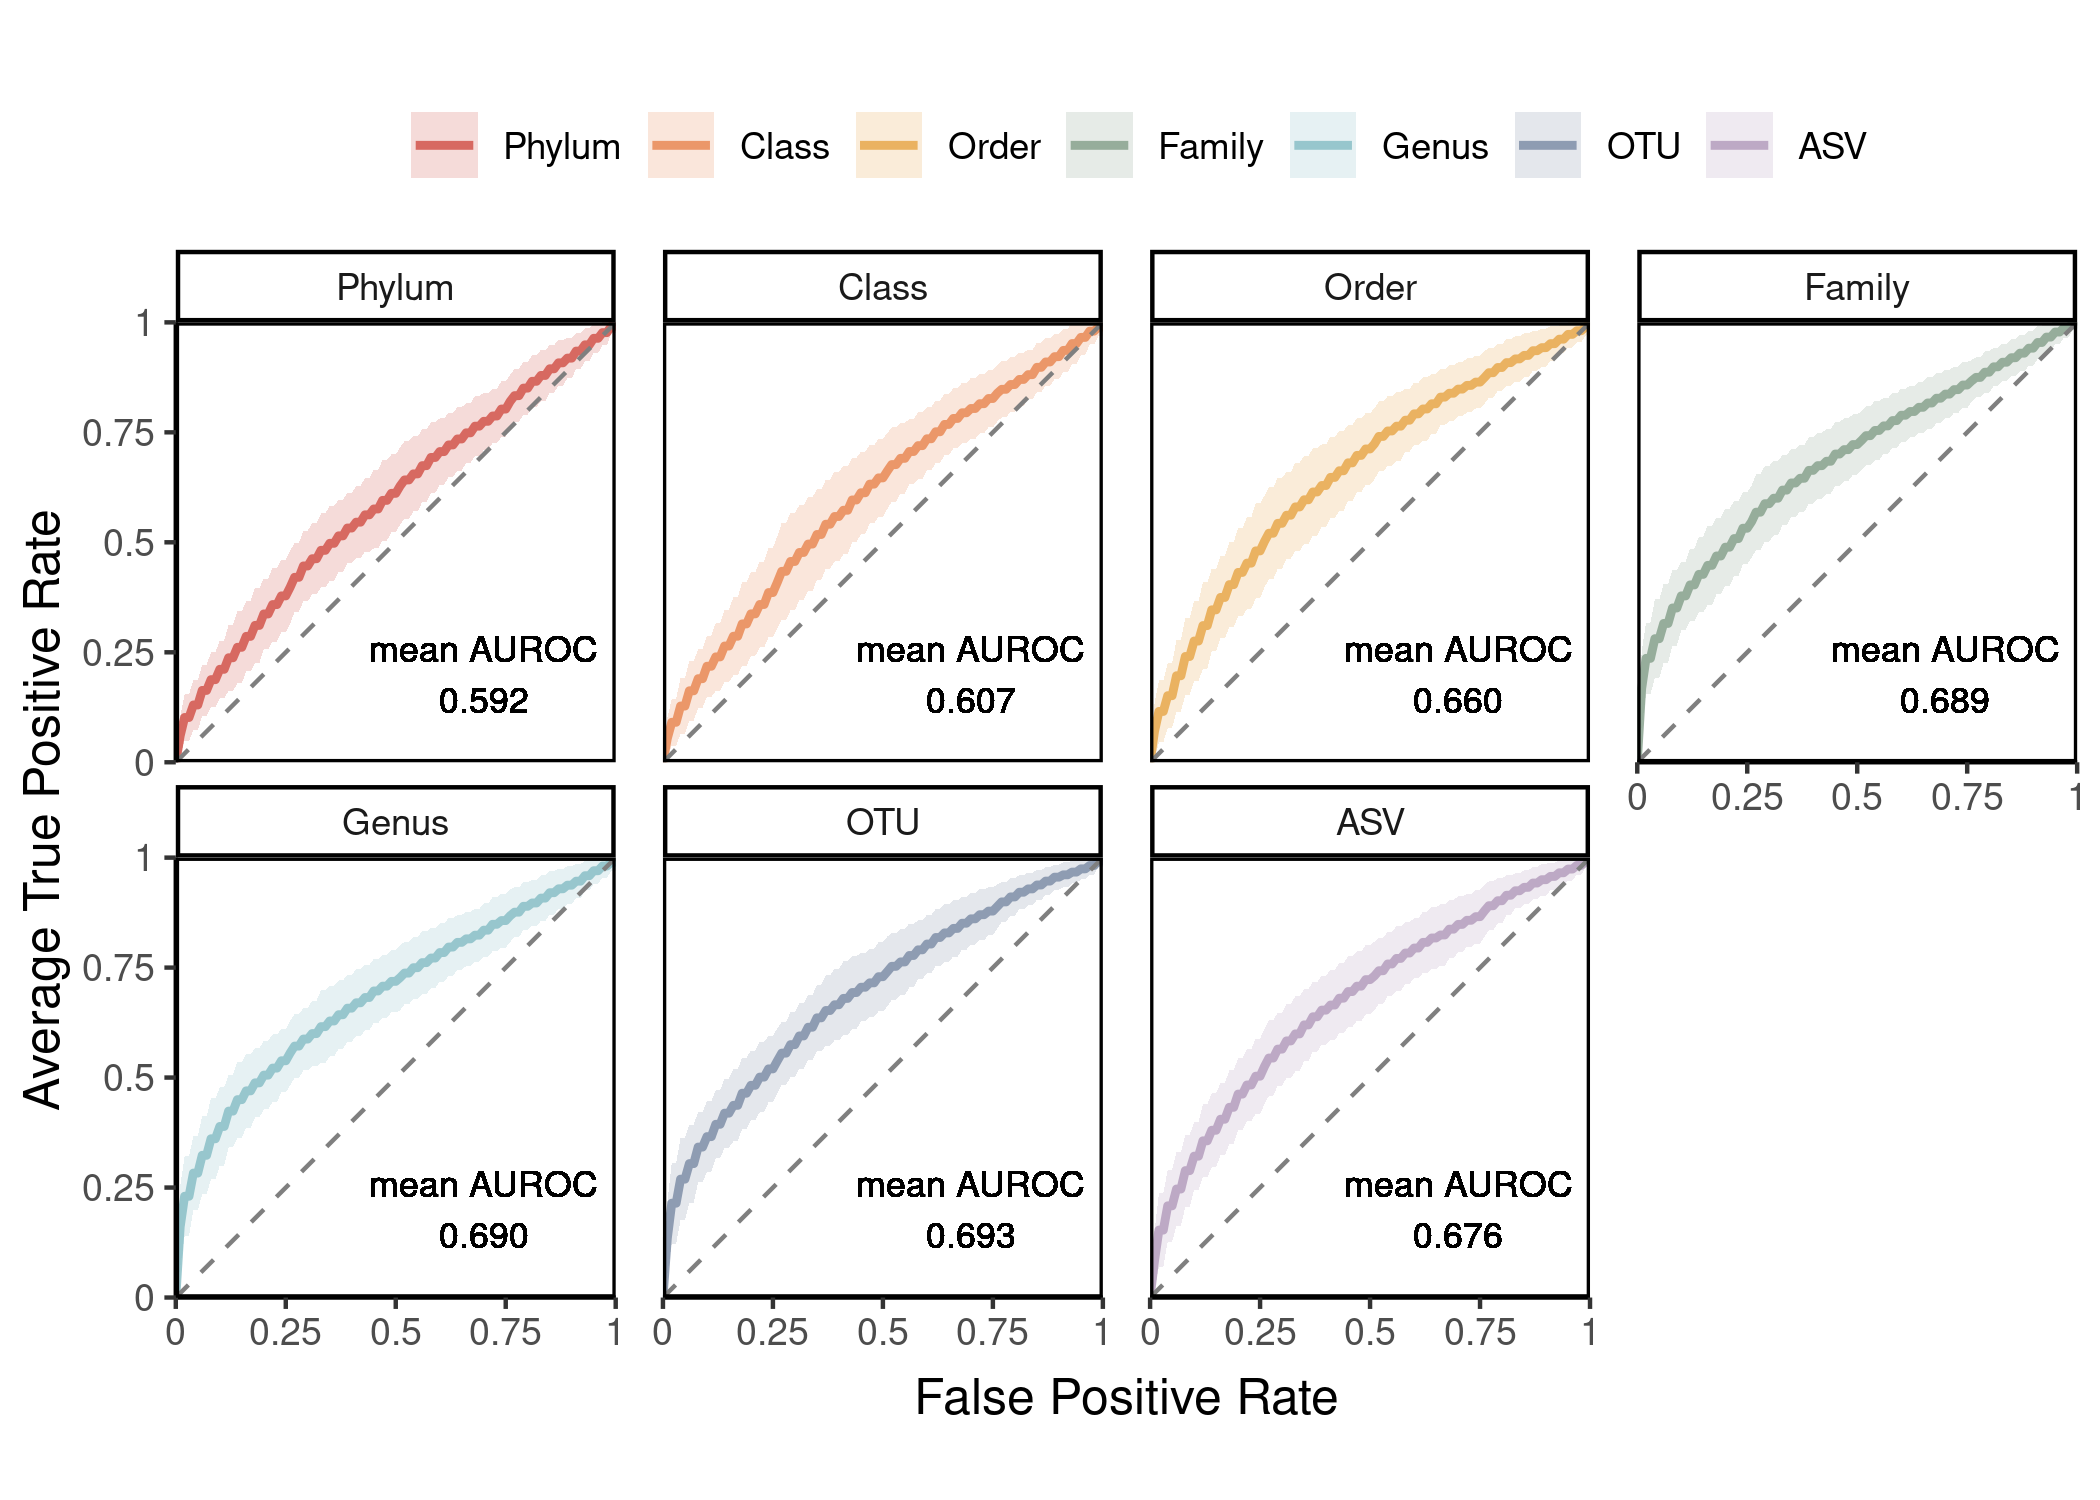
\includegraphics{figure_s2.png}\{height=``50\%''\}

\textbf{Supplemental Figure 2: Averaged ROC curves.} ROC curves with
averaged true positive rate (or sensitivity) across the 100 iterations
of the random forest model. The shaded region represents the standard
deviation form the mean. Dashed line represents an AUROC of 0.5, which
is equivalent to random classification. The mean AUROC for each
taxonomic level is printed on the bottom right of the plot.

\newpage

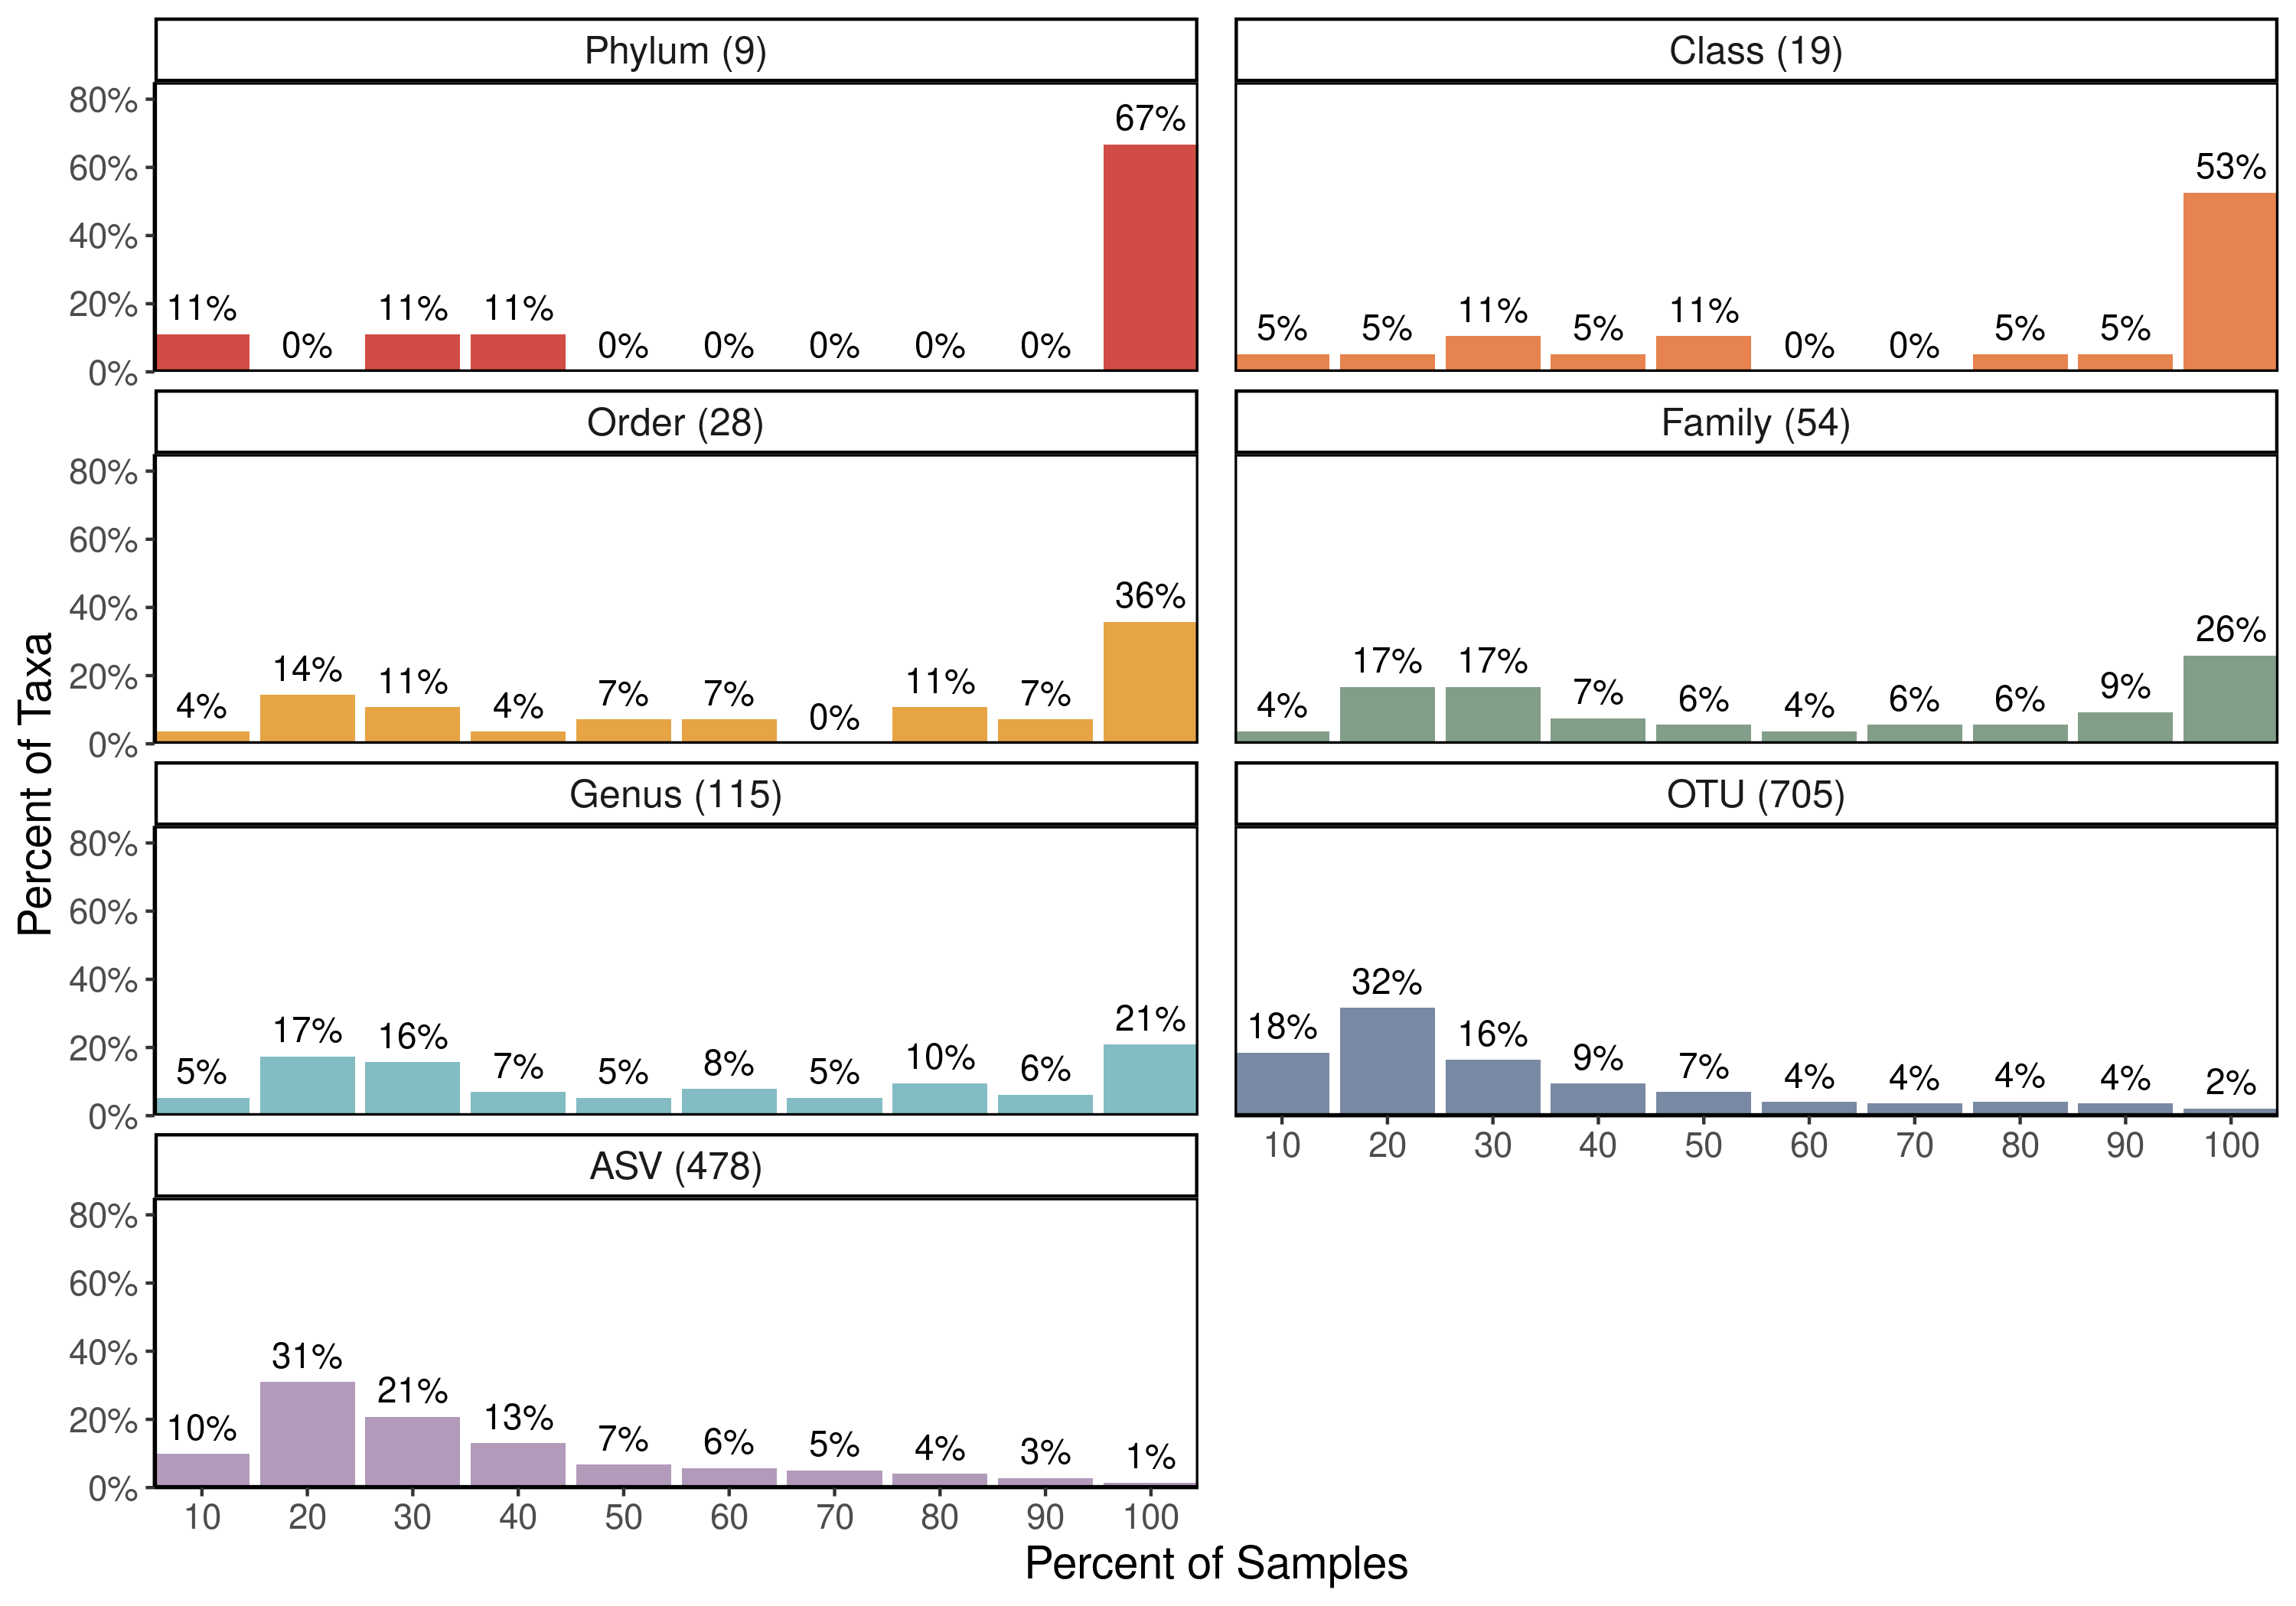
\includegraphics{figure_s3.png}\{height=``45\%''\}\\\textbf{Supplemental
Figure 3: Prevalence of Taxa in Samples.} Distribution of the prevalence
of taxa across samples at each taxonomic level. Percent of samples is
split into 10 groups where the first is for taxa present in 0 to 10\% of
samples, then \textgreater{}10\% to 20\% of samples, and so on. The
total number of taxa for each taxonomic level after preprocessing is in
parenthesis next to the title of the plot (or the name of the taxonomic
level).

\newpage

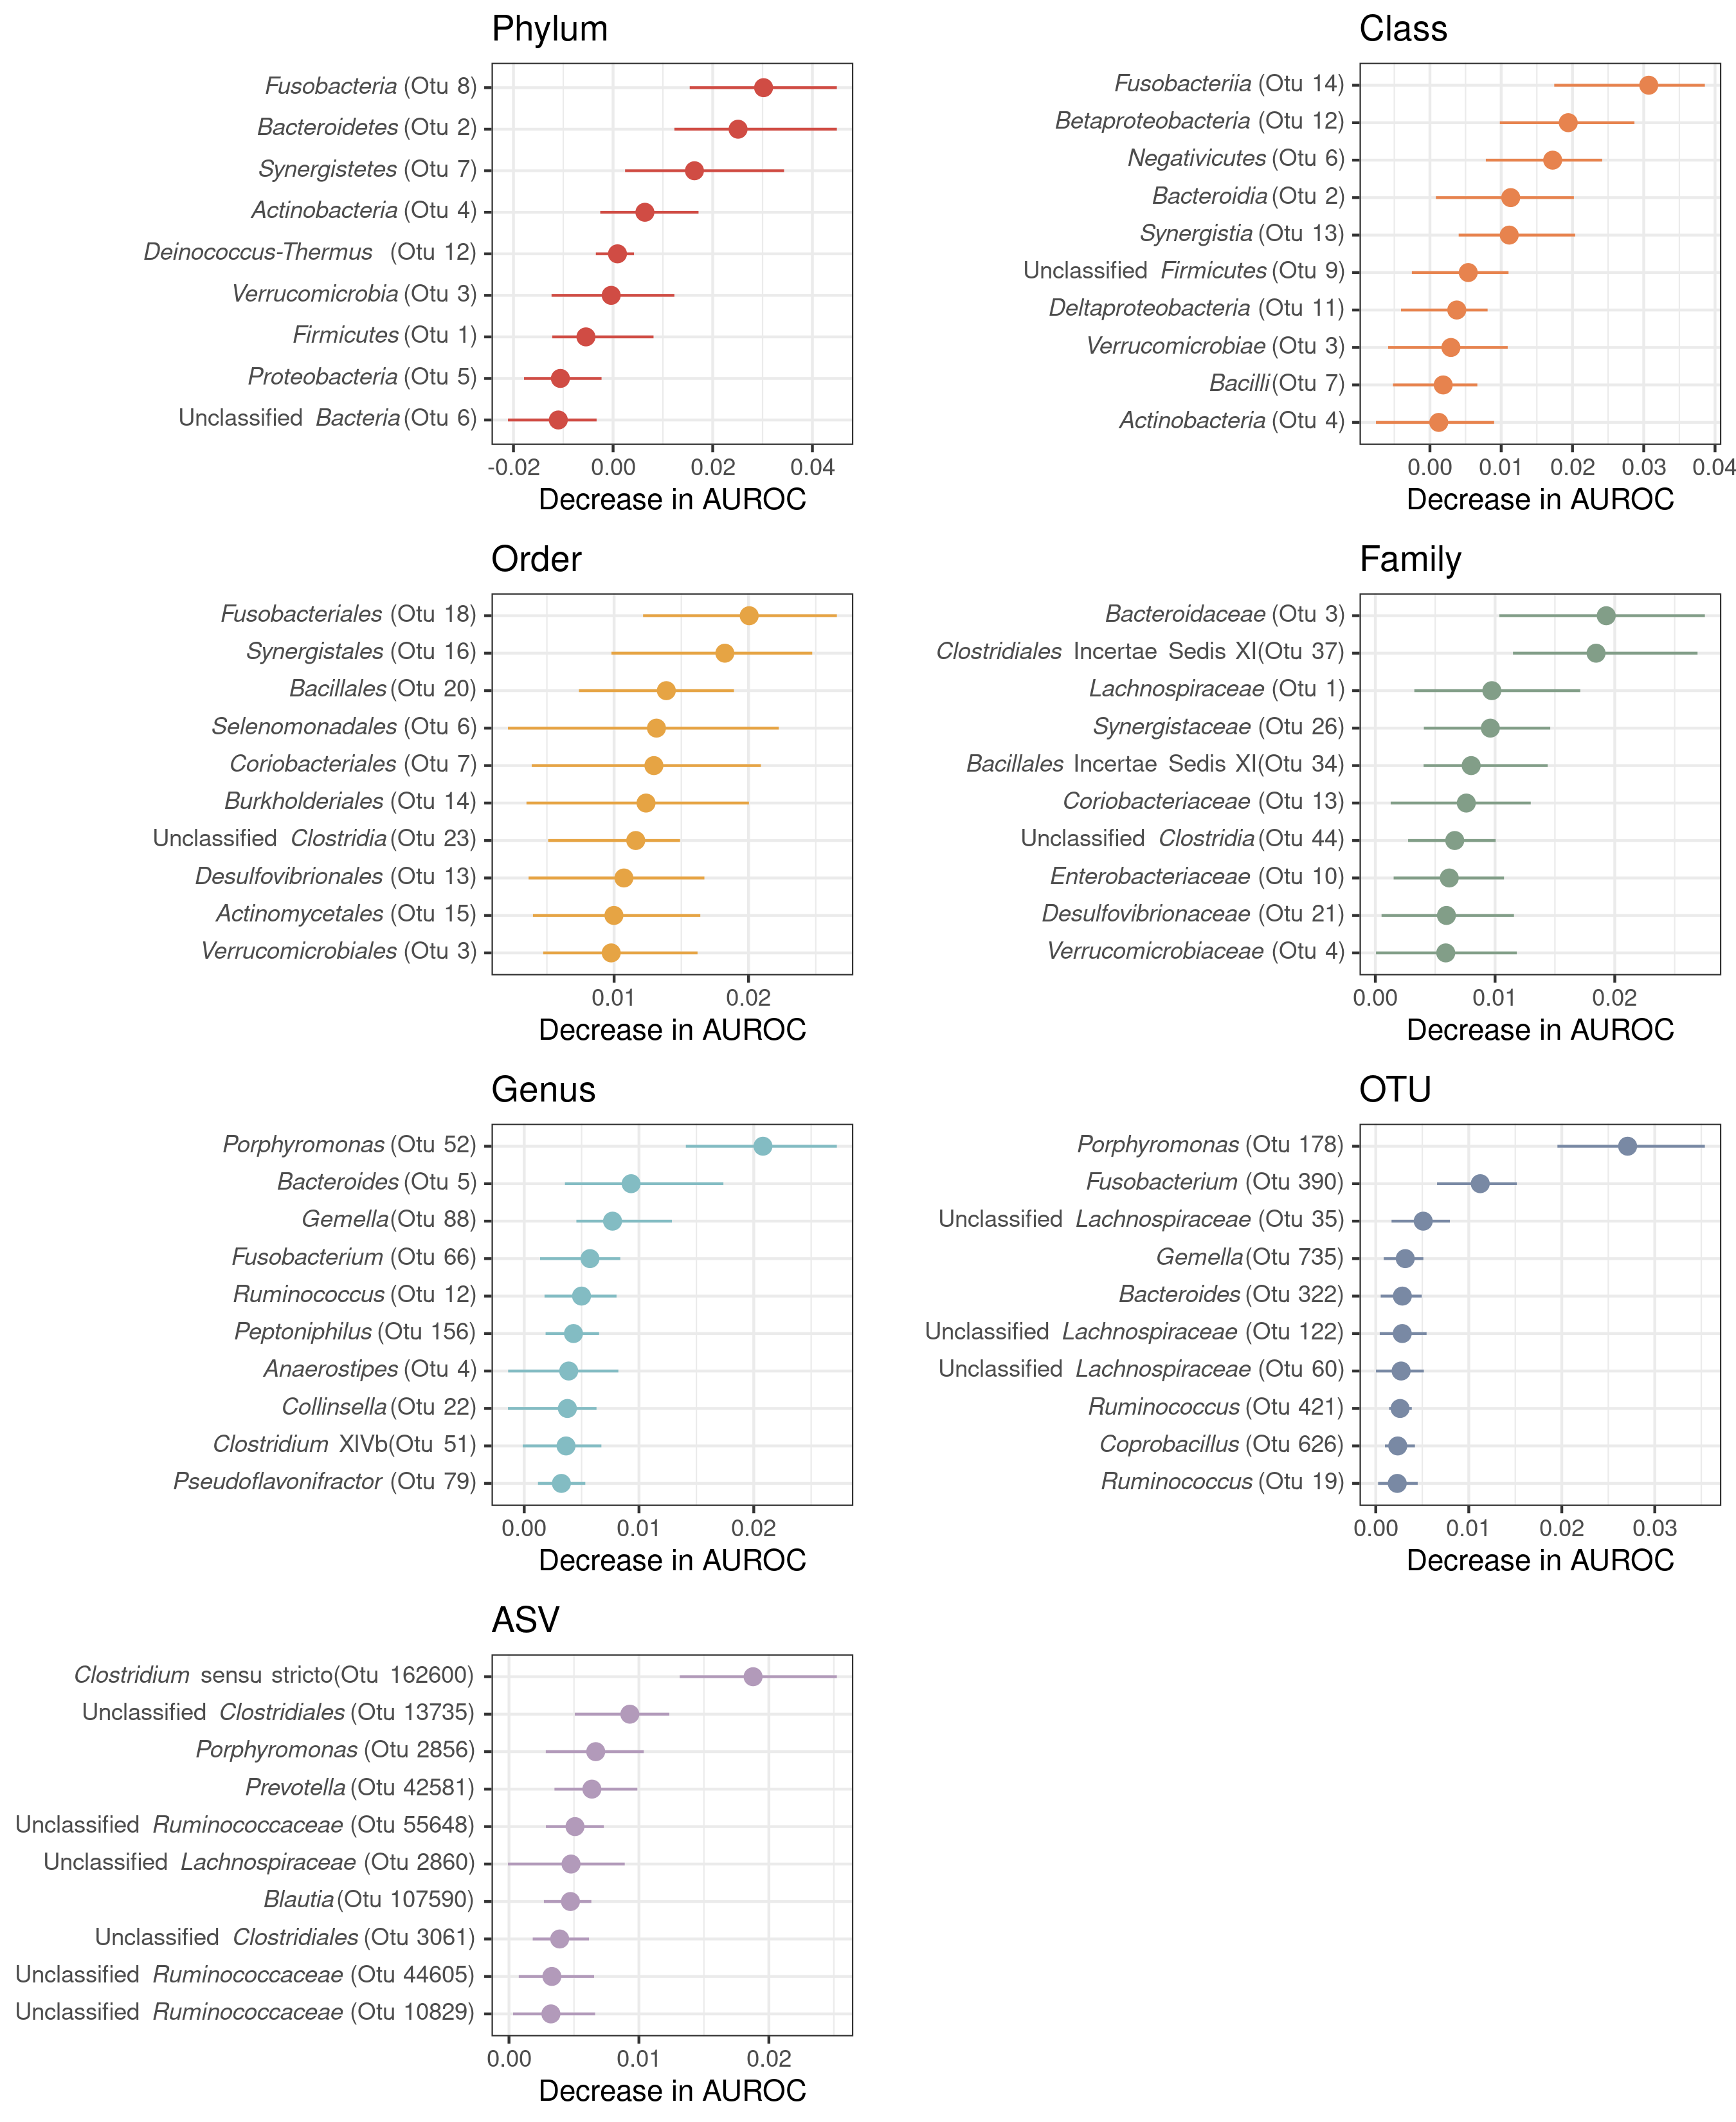
\includegraphics{figure_s4.png}\{height=``85\%''\}\\\textbf{Supplemental
Figure 4: Top 10 important taxa at each taxonomic level.} Summary of the
10 most important taxa for the random forest models at each taxonomic
level based on the average decrease in AUROC when the feature is
permuted. Dot represents the mean decrease in AUROC and the lines
extending from the dot represent the standard deviation from the mean.

1. \textbf{{Siegel} R}, \textbf{{Miller} K}, \textbf{{Sauer} A},
\textbf{{Fedewa} S}, \textbf{{Butterly} L}, \textbf{{Anderson} J},
\textbf{{Cercek} A}, \textbf{{Smith} R}, \textbf{{Jemal} A}. 2020.
Colorectal cancer statistics, 2020. CA: A Cancer Journal for Clinicians
\textbf{70}:145--164.
doi:\href{http://dx.doi.org/https://doi.org/10.3322/caac.21601}{https://doi.org/10.3322/caac.21601}.

2. \textbf{{García} G}, \textbf{{Z} A}. 2011. Factors influencing
colorectal cancer screening participation. Gastroenterology Research and
Practice \textbf{2012}:e483417.
doi:\href{http://dx.doi.org/10.1155/2012/483417}{10.1155/2012/483417}.

3. \textbf{{Zackular} J}, \textbf{{Rogers} M}, \textbf{{Ruffin} M},
\textbf{{Schloss} P}. 2014. The human gut microbiome as a screening tool
for colorectal cancer. Cancer Prevention Research \textbf{7}:1112--1121.
doi:\href{http://dx.doi.org/10.1158/1940-6207.CAPR-14-0129}{10.1158/1940-6207.CAPR-14-0129}.

4. \textbf{{Zeller} G}, \textbf{{Tap} J}, \textbf{{Voigt} A},
\textbf{{Sunagawa} S}, \textbf{{Kultima} J}, \textbf{{Costea} P},
\textbf{{Amiot} A}, \textbf{{Böhm} J}, \textbf{{Brunetti} F},
\textbf{{Habermann} N}, \textbf{{Hercog} R}, \textbf{{Koch} M},
\textbf{{Luciani} A}, \textbf{{Mende} D}, \textbf{{Schneider} M},
\textbf{{Schrotz-King} P}, \textbf{{Tournigand} C}, \textbf{{Nhieu} J},
\textbf{{Yamada} T}, \textbf{{Zimmermann} J}, \textbf{{Benes} V},
\textbf{{Kloor} M}, \textbf{{Ulrich} C}, \textbf{{Doeberitz} M},
\textbf{{Sobhani} I}, \textbf{{Bork} P}. 2014. Potential of fecal
microbiota for early-stage detection of colorectal cancer. Molecular
Systems Biology \textbf{10}:766.
doi:\href{http://dx.doi.org/10.15252/msb.20145645}{10.15252/msb.20145645}.

5. \textbf{{Callahan} B}, \textbf{{McMurdie} P}, \textbf{{Holmes} S}.
2017. Exact sequence variants should replace operational taxonomic units
in marker-gene data analysis. The ISME Journal \textbf{11}:2639--2643.
doi:\href{http://dx.doi.org/10.1038/ismej.2017.119}{10.1038/ismej.2017.119}.

6. \textbf{{Topçuo{ğ}lu} B}, \textbf{{Lesniak} N}, \textbf{{Ruffin} M},
\textbf{{Wiens} J}, \textbf{{Schloss} P}. 2020. A framework for
effective application of machine learning to microbiome-based
classification problems. mBio \textbf{11}.
doi:\href{http://dx.doi.org/10.1128/mBio.00434-20}{10.1128/mBio.00434-20}.

7. \textbf{{Schloss} P}, \textbf{{Westcott} S}, \textbf{{Ryabin} T},
\textbf{{Hall} J}, \textbf{{Hartmann} M}, \textbf{{Hollister} E},
\textbf{{Lesniewski} R}, \textbf{{Oakley} B}, \textbf{{Parks} D},
\textbf{{Robinson} C}, \textbf{{Sahl} J}, \textbf{{Stres} B},
\textbf{{Thallinger} G}, \textbf{{Van Horn} D}, \textbf{{Weber} C}.
2009. Introducing mothur: Open-source, platform-independent,
community-supported software for describing and comparing microbial
communities. Applied and Environmental Microbiology
\textbf{75}:7537--7541.
doi:\href{http://dx.doi.org/10.1128/AEM.01541-09}{10.1128/AEM.01541-09}.

8. \textbf{{Topçuo{ğ}lu} B}, \textbf{{Lapp} Z}, \textbf{{Sovacool} K},
\textbf{{Snitkin} E}, \textbf{{Wiens} J}, \textbf{{Schloss} P}. 2021.
mikropml: User-friendly r package for supervised machine learning
pipelines. Journal of Open Source Software \textbf{6}:3073.
doi:\href{http://dx.doi.org/10.21105/joss.03073}{10.21105/joss.03073}.

9. \textbf{{Lobo} J}, \textbf{{Jiménez-Valverde} A}, \textbf{{Real} R}.
2008. AUC: a misleading measure of the performance of predictive
distribution models. Global Ecology and Biogeography
\textbf{17}:145--151.
doi:\href{http://dx.doi.org/10.1111/j.1466-8238.2007.00358.x}{10.1111/j.1466-8238.2007.00358.x}.

10. \textbf{{Eren} A}, \textbf{{Maignien} L}, \textbf{{Sul} W},
\textbf{{Murphy} L}, \textbf{{Grim} S}, \textbf{{Morrison} H},
\textbf{{Sogin} M}. 2013. Oligotyping: differentiating between closely
related microbial taxa using 16S rRNA gene data. Methods in Ecology and
Evolution \textbf{4}:1111--1119.
doi:\href{http://dx.doi.org/10.1111/2041-210X.12114}{10.1111/2041-210X.12114}.

11. \textbf{{Eren} A}, \textbf{{Morrison} H}, \textbf{{Lescault} P},
\textbf{{Reveillaud} J}, \textbf{{Vineis} J}, \textbf{{Sogin} M}. 2015.
Minimum entropy decomposition: Unsupervised oligotyping for sensitive
partitioning of high-throughput marker gene sequences. The ISME Journal
\textbf{9}:968--979.
doi:\href{http://dx.doi.org/10.1038/ismej.2014.195}{10.1038/ismej.2014.195}.

12. \textbf{{Schloss} P}. Amplicon sequence variants artificially split
bacterial genomes into separate clusters. mSphere \textbf{6}:e00191--21.
doi:\href{http://dx.doi.org/10.1128/mSphere.00191-21}{10.1128/mSphere.00191-21}.

13. \textbf{{Baxter} N}, \textbf{{Ruffin} M}, \textbf{{Rogers} M},
\textbf{{Schloss} P}. 2016. Microbiota-based model improves the
sensitivity of fecal immunochemical test for detecting colonic lesions.
Genome Medicine \textbf{8}:37.
doi:\href{http://dx.doi.org/10.1186/s13073-016-0290-3}{10.1186/s13073-016-0290-3}.

14. \textbf{{Quast} C}, \textbf{{Pruesse} E}, \textbf{{Yilmaz} P},
\textbf{{Gerken} J}, \textbf{{Schweer} T}, \textbf{{Yarza} P},
\textbf{{Peplies} J}, \textbf{{Glöckner} F}. 2013. The sILVA ribosomal
rNA gene database project: improved data processing and web-based tools.
Nucleic Acids Research \textbf{41}:D590--D596.
doi:\href{http://dx.doi.org/10.1093/nar/gks1219}{10.1093/nar/gks1219}.

15. \textbf{{Callahan} B}, \textbf{{McMurdie} P}, \textbf{{Rosen} M},
\textbf{{Han} A}, \textbf{{Johnson} A}, \textbf{{Holmes} S}. 2016.
DADA2: High-resolution sample inference from illumina amplicon data.
Nature Methods \textbf{13}:581--583.
doi:\href{http://dx.doi.org/10.1038/nmeth.3869}{10.1038/nmeth.3869}.

\end{document}
